\chapter{Background}
\label{background}

%------------------------------------------------------------------

\section{Rhetoric and Argumentation}
\label{background:rhetoric}
Rhetoric is often used in modern parlance as a pejorative to describe persuasive language that lacks substance, or containing empty or insincere promises; formally, however, it refers to the art of persuasion, whether spoken or written. In particular, it focuses on the act tailoring one's argument to the situation at hand based on knowledge of events and, crucially, knowledge of the audience \citep{Corbett1999}.

\subsection{Modes of Persuasion}
Aristotle, in his treatise on rhetoric, described three ``persuasive modes'' that can be employed in an attempt to sway an audience: through the words that are used (\textit{logos}), through the character of the rhetor or their opponent (\textit{ethos}), and through the emotions of the audience (\textit{pathos}) \citep{Kennedy1991}. These modes may be applied individually, or in conjunction with one another. \textit{Logos} describes an appeal to logic or reason. This is the method by which one might rationalise a position, often backing it up with evidence or statistics. It is important to note that, when enacting \textit{logos}, it is not strictly necessary for the logic to be sound, or the evidence provided to be factual -- it can be warped to fit a particular purpose, or even outright fabricated (however, this will usually also invoke another of the modes described below). The key element is that it appears to be reasonable and thus, appeals to an audience's sense of reason \citep{Kennedy1991, Braet1992}. \textit{Ethos} is an appeal a person's character or sense of ethics and morals. This can be used in an attempt to strengthen the position of the rhetor's argument or to weaken their opponent's position. For example, if a rhetor can state that they are an expert in the field that they are debating then it is likely their audience will lend their argument more credence than if they were a novice. This specific case is known as an argument from authority, or \textit{argumentum ab auctoritate} \citep{Kennedy1991, Braet1992}. Similarly, an argument can be made that attacks an opponents position indirectly, by attacking their credentials rather than refuting their claims (\textit{argumentum ad hominem}). Although such an argument is not logically sound (and constitutes a fallacy), it is still often used in practice and in certain circumstances is a viable (and often effective, if somewhat underhand) means of persuading an audience \citep{walton1987, Budzynska2012}. Finally, \textit{pathos} is an appeal to emotion, whereby an attempt is made to evoke a particular feeling in an audience in the hope that this will influence their opinion on a position. This can be done in both positive and negative terms. For example, flattering an audience, or promising them a boon, can shift them towards accepting a particular course of action. On the other hand, threatening them with the potentially undesirable consequences of their actions can cause them to reconsider even if these consequences are unlikely or, indeed, impossible. A classic example is the appeal to fear (\textit{argumentum ad metum}) \citep{Kennedy1991, Braet1992}.


\subsection{Dialectic and Eristic Argument}
\label{background:rhetoric:dialectic}
The terms dialectic and eristic were coined in Ancient Greece to describe modes of argumentation with different goals and were popularised in Plato's \textit{Republic} \citep{Bloom1991}. A dialectic argument takes the form of two or more parties engaged in rational discourse with the aim of either discovering the particular truth behind a matter, or formulating a solution or resolution for a set of circumstances \citep{kerferd1981}. For example, an academic presenting their findings and rationalising that they are indeed valid, given the rigorous methodology they have used and the weight of evidence this has provided is an example of a dialectic argument. Likewise, a peer reviewer that disagrees with the findings by pointing out a specific flaw in the experimental methodology and explaining how this should be resolved, is another example. The arguments tend to rely heavily on the mode of \textit{logos}. In contrast, an eristic argument is an argument in which there is no clear resolution in the minds of the participants: they are not motivated by solving a problem, or convincing their opponent, but to be victorious \citep{kerferd1981}. There may be different reasons for arguing in this vein, from quarrelling for its own sake as a form of catharsis \citep{Schneider2014}, to being seen to ``win'' the argument in the eyes of spectators \citep{Jorgensen1998}. As a result, these arguments chiefly favour the modes of \textit{ethos} and \textit{pathos}.

\TODO{Polemics} \citep{lemaitre2015}


\subsection{Modelling Argument}
\label{background:rhetoric:modelling}
There are many different models and frameworks used to capture particular aspects of argumentation. These aspects include notions of trust \citep[p.~752]{Wigmore1913}, focus on argument topic or chronology \citep{Klein2010} and the ability to demonstrate support for or refutation of other points in the structure \citep{Dung1995}. Some examples are discussed below, with respect to their technical structure, their influence in the field and their practical applications.


\subsubsection{Toulmin Model}
Toulmin developed his model from the school of philosophy in the 1950s as a means of demonstrating an approach to practical (rather than theoretical) argumentation, by attempting to show the internal structure (and thus, consistency) of an argument \citep{Toulmin1958}. The general form of Toulmin's argument, shown in Figure \ref{figure:toulmin:general}, follows the structure of a \textit{claim}, or conclusion, that is backed up with generally agreed upon facts (the \textit{data}). The \textit{claim} can be \textit{qualified} (``definitely'', ``maybe'', ``probably'', etc.) and any potential \textit{rebuttals} accounted for. Then, key to the Toulmin model, the \textit{claim} and \textit{data} are connected using either an implicit or explicit \textit{warrant}, or justification -- this can then be supported by a particular \textit{backing} \citep[p.~347-350]{Verheij2005}. A specific example can be seen in Figure \ref{figure:toulmin:specific}, which shows an argument reasoning that Alice is a British citizen. Toulmin's model has been a particularly influential piece of work and has had an impact of decades of argumentation research  in fields as far ranging as law, rhetoric and education (\citealp[p.~8-10]{Newman1992}; \citealp[p.~5, 12]{Schneider2013}). However, there has been discussion as to the effectiveness of different aspects of the framework. In its favour, the means of explicitly stating the connecting warrant (and associated backing) can improve cross domain discourse. On the other hand, because models themselves are focused towards internal structure, there is no criteria for modelling overall structure (such as a group of arguments that refutes or support one another's claims). There is also no concept of resolving an argument (for example, on the grounds of logic or value); although this may have been by design, it negates the possibility of evaluating the strength of a given argument (\citealp[p.~349-350]{Newman1992}; \citealp[p.~5, 12]{Verheij2005}). Among other applications, the Toulmin model has been incorporated into the Argument Model Ontology\footnote{http://www.essepuntato.it/2011/02/argumentmodel}, an OWL ontology to allow classification of academic arguments. This is used in conjunction with CiTO, an ontology for factually and rhetorically categorising citations \citep[p.~8]{Peroni2012}.

\begin{figure}[H]
\begin{displaymath}
\xymatrix{
\mbox{\textit{Data}} \ar[rr] && \mbox{So, \textit{(Qualifier) Claim}} \ar[d]\\
& \mbox{Because \textit{Warrant}} \ar[u]& \mbox{Unless \textit{Rebuttal}}\\
& \mbox{Due to \textit{Backing}} \ar[u]&
}\\
\end{displaymath}
\caption{General form of Toulmin's diagram \citep[p.~104]{Toulmin1958}}
\label{figure:toulmin:general}
\end{figure}



\begin{figure}[H]
\begin{displaymath}
\xymatrix{
\mbox{\parbox[t]{0.2\linewidth}{Alice was\\born in Bermuda}} \ar[rr] & & \mbox{\parbox[t]{0.2\linewidth}{So, Alice is (presumably) a British citizen}} \ar[d]  \\
& \mbox{\parbox[t]{0.2\linewidth}{Because a person\\born in Bermuda\\will be a British\\citizen}} \ar[u]& \mbox{\parbox[t]{0.2\linewidth}{Unless both of\\Alice's parents\\were aliens (etc.)}} \\
&&&\\
& \mbox{\parbox[t]{0.2\linewidth}{Due to the\\British Overseas\\Territories Act 2002}} \ar[u]&
}\\
\end{displaymath}
\caption{Example usage of Toulmin's diagram \citep[p.~105]{Toulmin1958}, examining whether Alice is a British citizen}
\label{figure:toulmin:specific}
\end{figure}

\subsubsection{Information-Based Issue Systems}
Information-Based Issue System (IBIS) models are a particular type of dialectic process originally designed to aid in solving so-called ``wicked problems'' \citep{Kunz1970} -- problems of social policy to which there is no clear definition, methodology or even end-goal \citep{Rittel1973}. IBIS models are represented as trees, made up of four different types of node. Firstly, \textit{Issues} represent the problems that need to be solved, or questions that must be answered. Generally, there is one ``root'' \textit{Issue} to be deliberated, but other sub-\textit{Issues} can be created as necessary during the reasoning process. \textit{Ideas} are proposed solutions or answers to these \textit{Issues}, and each \textit{Idea} can then be weighted positively or negatively using \textit{Arguments For} and \textit{Arguments Against}. IBIS models have seen wide usage in the field of design rationale and cognitive ergonomics where the assimilation of collective knowledge is required to solve problems \citep{Conklin1987, Aurisicchio2013}. An example usage of an IBIS model is shown in Figure \ref{figure:ibis}. Because of its dialectic context, the application of IBIS models is ideal when two or more parties are trying to resolve a complex problem, especially if they have differing (or even opposing) stakes. As might be expected, there are many IBIS-like systems used in system-design and knowledge aggregation. Delibatorium\footnote{http://deliberatorium.mit.edu} is a tool, developed by \citet{Klein2010} of MIT, that uses an IBIS approach to solving challenging problems such as \textit{``Is carbon offsetting a good idea?''}. The IBIS approach is invoked to aid the collaboration of large amounts of people separated across space and time by preserving a topic-centric (rather than time-centric) structure. IBIS structures have also been included in an extension to the SIOC ontology devoted to representing argumentation\footnote{http://rdfs.org/sioc/argument}. This ontology uses the IBIS notation of \textit{Issues} and \textit{Ideas} to formalise the process of solving a problem over social media \citep{Lange2008}.

\begin{figure}[H]
\begin{center}
\begin{tikzpicture}[node distance=3.5cm,>=stealth',bend angle=10]

	\tikzstyle{rect}=[
		rectangle,
		thick,
		draw=black,
  		fill=white
  	]
	

	\node [rect, font=\footnotesize] (A) [] {\parbox{0.2\textwidth}{\textbf{\textit{Issue:}}\\Is Alice a British citizen?}};

	\node [rect, font=\footnotesize] (B) [above right=16mm] {\parbox{0.2\textwidth}{\textbf{\textbf{\textit{Idea:}}}\\Alice would be a British citizen if she had a British passport}};
	\node [rect, font=\footnotesize] (C) [below right=16mm] {\parbox{0.2\textwidth}{\textbf{\textit{Idea:}}\\Alice would be a British citizen if she was born in a British territory}};
	

	\node [rect, font=\footnotesize] (E) [right of=B] {\parbox{0.2\textwidth}{\textbf{\textit{Disagreement:}}\\Alice does not hold (any) passport}};
	
	\node [rect, font=\footnotesize] (F) [right of=C] {\parbox{0.2\textwidth}{\textbf{\textit{Agreement:}}\\Alice was born in Bermuda (a British Overseas Territory)}};
	\node [rect, font=\footnotesize] (G) [below right of=C] {\parbox{0.2\textwidth}{\textbf{\textit{Disagreement:}}\\Being born in overseas territory makes one an Overseas Citizen}};
	
	\node [rect, font=\footnotesize] (H) [right of=F] {\parbox{0.2\textwidth}{\textbf{\textit{Issue:}}\\Alice might be disqualified if her parents are aliens}};
	
	\draw[post] (A)--(B)  ;
	\draw[post] (A)--(C)  ;
	
	\draw[post] (B)--(E)  ;
	
	\draw[post] (C)--(F)  ;
	\draw[post] (C)--(G)  ;
	
	\draw[post] (F)--(H)  ;
      
\end{tikzpicture}
\end{center}
\caption{Example usage of an IBIS model, examining whether Alice is a British citizen}
\label{figure:ibis}
\end{figure}


\subsubsection{Wigmore's Chart}
``Wigmore's chart'', conceived in 1913, is a means of recording argumentation originally devised for use in legal trials. The chart models the chain of interactions between competing arguments from both participants and can be used to evaluate the overall conclusion that should be drawn \citep[p.~751]{Wigmore1913}. It takes the form of a directed graph where each node represents a particular fact. The shape of each node relates to the nature of the assertion; squares represent testimony given under oath; a triangle represent an explanation of or support for the node it ``points'' to; an open angle refutes the argument it points to and all other assertions (such as claims, physical evidence or related legal statutes) are represented by circles. These can additionally be marked to denote arguments by the defence or prosecution, but are not discussed here for clarity \citep{Chalamish2011, Chalamish2013}. Symbols relate further information about the nature of these assertions: an infinity symbol ($\infty$) states that a node denotes sensory evidence that may be (re)produced in court; a pilcrow (\P) denotes an assertion that can be taken as fact with no further evidence (such as a precedence case); a lack of a symbol shows that the claim is implied from further reasoning in the graph. In addition, Wigmorean analysis can incorporate the notions of \textit{strong belief} ($\bullet\bullet$), \textit{belief}($\bullet$) \textit{doubt} (?) \textit{disbelief} ($\circ$) and \textit{strong disbelief} ($\circ\circ$) (\citealp[p.~751-756]{Wigmore1913}; \citealp{Goodwin2000}). Little is known about precisely how often this type of analysis is used manually, although it is thought that it is carried out in courthouses around the world \citep{Chalamish2011}. However, efforts are being made to automate the process by parsing the natural language propositions made in court and transforming these into a Wigmore diagram to aid judges, barristers and juries in their deliberations \citep{Chalamish2013}.

\begin{figure}[h!]

\makeatletter
\newif\ifpgfshapebaselesstrianglehasinline
\newif\ifpgfshapebaselesstriangleclose
\pgfkeys{/pgf/.cd,
  baseless triangle apex angle/.style={/pgf/isosceles triangle apex angle=#1},
  baseless triangle inline/.is if=pgfshapebaselesstrianglehasinline,
  baseless triangle has base/.is if=pgfshapebaselesstriangleclose
}

\pgfdeclareshape{baseless triangle}{
  % Copy some stuff from the isosecles triangle
  \inheritsavedanchors[from={isosceles triangle}]
  \inheritanchor[from={isosceles triangle}]{center}
  \inheritanchor[from={isosceles triangle}]{north}
  \inheritanchor[from={isosceles triangle}]{south}
  \inheritanchor[from={isosceles triangle}]{east}
  \inheritanchor[from={isosceles triangle}]{west}
  \inheritanchorborder[from={isosceles triangle}]
  \backgroundpath{%
    % The isoceles triangle defines lots of parameters
    % in the \trianglepoints macro.
        \trianglepoints%
        {%
            \pgftransformshift{\centerpoint}%
            \pgftransformrotate{\rotate}%
            % This bit is a bit of a kludge to ensure the inline
            % is at the top of the figure.
            \pgftransformyscale{cos(\rotate)}%
            \pgfpathmoveto{\lowerleft}%
            \pgfpathlineto{\apex}%
            \pgfpathlineto{\lowerleft\pgf@y=-\pgf@y}%
            % Close the base?
            \ifpgfshapebaselesstriangleclose%
              \pgfpathclose%
            \fi%
            % Draw the inline?
            \ifpgfshapebaselesstrianglehasinline
              \pgfpointdiff{\lowerleft}%
                 {\pgfpointlineattime{0.125}{\lowerleft}{\lowerleft\pgf@y=-\pgf@y}}%
                \pgfgetlastxy{\x}{\y}%
                \pgfmathveclen{\x}{\y}%
                \let\inlineshift=\pgfmathresult%
            % Calculate where the inline hits the sloped line of the triangle.
            \pgfmathparse{\inlineshift/2/sin(\pgfkeysvalueof{/pgf/isosceles triangle apex angle}/2)}%
            \let\inlineendshift=\pgfmathresult
            \pgfpathmoveto{\pgfpointadd{\pgfpoint{0pt}{-\inlineshift}}{\lowerleft}}%
            \pgfpathlineto{\pgfpointlineatdistance{\inlineendshift}{\apex}{\lowerleft}\pgf@y=-\pgf@y}%
        \fi%
    }
    }
}

\begin{center}
\begin{tikzpicture}[node distance=1.6cm,>=stealth',bend angle=45]

	\tikzstyle{circ}=[
		circle,
		thick,
		draw=black,
		fill=white,
		minimum size=6mm
	]

	\tikzstyle{rect}=[
		rectangle,
		thick,
		draw=black,
  		fill=white,
  		minimum size=6mm
  	]
  			  
	\tikzset{
		support/.style={
			regular polygon,
			regular polygon sides=3,
			shape border rotate=90,
			thick,
        	draw=black,
	        fill=white,
        	minimum height=6mm,
        	node distance=0.6cm
    	}
    }
    
    \tikzset{	
		refute/.style={
	    	draw,
	    	thick,
	    	baseless triangle,
 	   		baseless triangle apex angle=60,
 	   		shape border rotate=180,
 	   		baseless triangle inline=false,
 	   		baseless triangle has base=false,
 	   		node distance=0.6cm
  		}
  	}



	\node [circ,tokens=1] (1) [label=above right:$_1$] {};
	
	\node [circ,tokens=2] (2) [right of=1,label=above right:$_2$,label=below right:$\infty$] {};
	\node [support] 	  (2a)[left of=2] {};	
	
	\node [circ,tokens=1] (3) [below left of=1,label=above right:$_3$] {};	
	\node [circ,tokens=2] (4) [below of=3,label=above right:$_4$,label=below right:\footnotesize{\P}] {};

	\node [circ,tokens=1] (5) [below right of=1,label=above right:$_5$] {};
	


	\node [rect,tokens=1] (6) [below of=5,label=above right:$_6$] {};	

	\node [circ] (7)  [right of=6,label=above right:$_7$] {$\circ$};
	\node [refute] (7a)  [left of=7] {};

	\draw[post] (3)-|(1)  ;
	\draw[post] (5)-|(1)  ;
	\draw[post] (4)--(3)  ;
	\draw[post] (6)--(5)  ;
	\draw[post] (2a)--(1)  ;
	\draw[post] (7a)--(6)  ;
	
 
      
\end{tikzpicture}
\end{center}

\begin{tabular}{l l}
\begin{minipage}{0.5\textwidth}
\begin{enumerate}
	\item[$^1$] \footnotesize{Alice is a British citizen}
	\item[$^2$] \footnotesize{Alice has a British passport}
	\item[$^3$] \footnotesize{A person born in a British territory will be a British citizen}
	\item[$^4$] \footnotesize{British Overseas Territories Act 2002}
\end{enumerate}
\end{minipage}

\begin{minipage}{0.5\textwidth}
\begin{enumerate}
	\item[$^5$] \footnotesize{Alice was born in Bermuda}
	\item[$^6$] \footnotesize{Alice's parents testify that she was born in Bermuda}
	\item[$^7$] \footnotesize{Alice's parents' testimony could be biased in her favour}
\end{enumerate}
\end{minipage}
\end{tabular}
\caption{Example Wigmore graph, examining whether Alice is a British citizen}
\label{figure:wigmore}
\end{figure}


\subsubsection{Dung's Framework}
Similar to Wigmore's method, Dung's framework (which uses the format of set theory) focuses on the aspect of arguments attacking, (implicitly) supporting and, ultimately, defeating one another \citep{Dung1995}. Dung defines an \textit{Argument Framework} as a pair such that $AF = \langle AR, attacks \rangle$ where $AR$ is a set of arguments $\left\{a_1, a_2, ..., a_n\right\}$ and $attacks$ is a binary relation such that $attacks \subseteq AR \times AR$. $attacks$ describes which arguments are ``defeated'' by one another: for example, if $a_1$ is the argument ``Alice is not a British citizen'' and $a_2$ is the argument ``Alice has a British passport'' then $(a_2, a_1) \in attacks$. The set of \textit{conflict free} arguments is a maximal set of arguments that do not attack each other. An argument $a_1$ is \textit{acceptable} with regard to a set of arguments $S$ if there is no argument $a_2$ that attacks $a_1$ that is not itself attacked by an argument in $S$. A set of arguments is \textit{admissible} if each argument is considered \textit{acceptable} with respect to the set. The maximal \textit{admissible} set is known as a \textit{preferred extension} \citep{Schneider2013}. 

\TODO{Other extensions}
There have been a number of extensions to this framework.
\citet{Bench-Capon2002} have extended this framework to incorporate the idea of ``value'' or principle to arguments. When circumstances arise such that two possible resolutions to a dispute are equally (logically) valid, different audiences will have differing preferences based on the principles they feel are most important. For example, say that two solutions for combating crime are put forward: reading the general public's private correspondence or an expensive social program of education and rehabilitation. If each has been proven to be equally effective, audiences that value minimisation of cost may favour the former whereas audiences that value individual privacy might choose the latter.
\citet{dunne2016heard} incorporated this to \TODO{FINISH}


\subsubsection{ASPIC}
\TODO{EXPAND THESE}

\subsubsection{ASPIC+}

\subsubsection{IMPACT structured consultation tool}
\TODO{THIS} \citep{wyner2011towards}

\subsubsection{The Argument Interchange Format}
The Argument Interchange Format (AIF) is a framework for representing argumentation as a directed graph \citep{Chesnevar2006}. Created as part of the Argument Web project \citep{Rahwan2007a}, which aims to link the concepts of natural language argumentation with abstract mathematical modelling (including capturing \textit{``linguistically sophisticated manoeuvres''} \citep{Bex2013}), the AIF is primarily a description, with specifications in a number of languages including RDF and SQL.

At its highest level, the AIF can be conceptually divided into an ``upper'' ontology and a ``forms'' ontology. The upper ontology consists of the building blocks of the argument structure, while the forms ontology applies context, for example, by differentiating between logical attacks based on faulty evidence, witness bias, or appeals to authority. The data, claims and conclusions that make up the argument are modelled by Information nodes (I-nodes). There can be no direct relationship between I-nodes. Instead, there must be an intermediary Scheme node (S-nodes). These S-nodes are subdivided into three applications: Rule of Inference Applications (RA-nodes), Conflict Applications (CA-nodes) and Preference Applications (PA-nodes). RA-nodes and CA-nodes simply denote an inference or conflict (logical or otherwise) between one or more pieces of information. PA-nodes, however, denote a preference of one piece of information over another. For example when discussing economics, while it may be difficult to logically prove the superiority of a regulated market over a free market, or vice-versa, the personal beliefs and preferences of proponent and opponent will feature heavily in their reasoning on such issues \citep{Bench-Capon2002}. This structure is displayed in Figure \ref{figure:ontologies:aif}.

\begin{figure}
\begin{center}
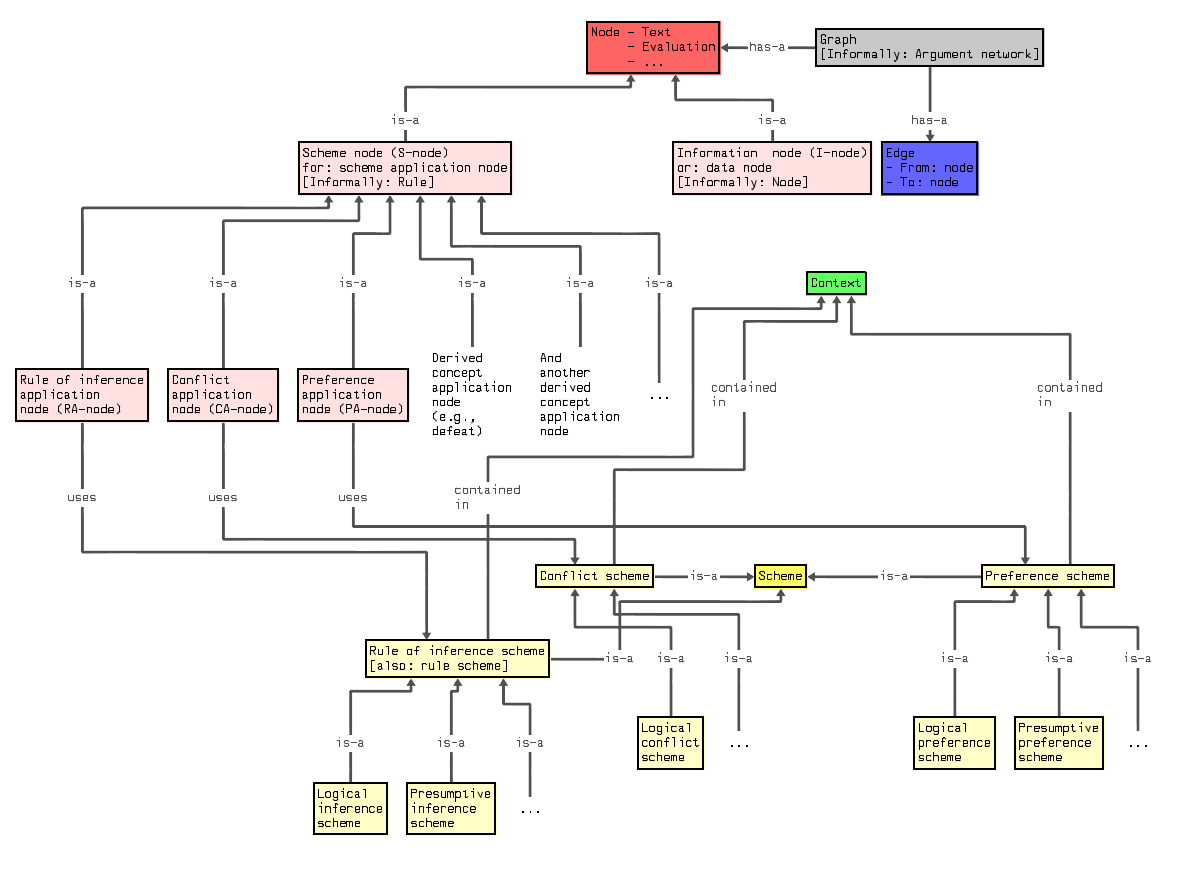
\includegraphics[scale=0.42]{./figures/ontologies/aif.png}
\caption{An overview of the AIF Ontology \citep{Chesnevar2006}}
\label{figure:ontologies:aif}
\end{center}
\end{figure}

\subsubsection{AIF+ and Inference Anchoring Theory}

\TODO{Expand details from IAT paper}


In their work on an extension to the AIF, dubbed the AIF+, Reed et al. build on the work of O'Keefe to differentiate between two separate notions of argumentation \citep{Benoit1992, Reed2008}: the first, which they term argument$_1$, is a logically constructed set of claims and evidence used to back these claims (or attack other claims), as in \textit{``Alice put forward her argument''}. The second, termed argument$_2$, refers to a dialogue -- the exchange of ideas and opinions between two or more people, as in \textit{``Alice and Bob were having an argument}. A result of this work was to introduce a new set of nodes. The first, a subset of I-nodes dubbed Locutions (L-nodes), model locutionary acts (or utterances) in an argument$_2$. That is, they record precisely what was said. The second, a subset of S-nodes dubbed Transition Applications (TA-nodes), represent transitions between L-nodes (with associated forms such as a challenge or response). Thirdly Illocutionary Applications (YA-nodes), also a subset of S-nodes, represent the ``illocutionary force'' and serve to link each argument$_1$ to the overall argument$_2$. Figure \ref{figure:graphs:aifplus} shows how this structure can be visualised. Consider the locution \textit{``All men are mortal, and Socrates is a man. Therefore, Socrates is mortal.''} The statement itself is modelled using the L-node on the rightmost side of the diagram. On the leftmost side is the core AIF structure, which show the premises formed as two I-nodes (\textit{``Socrates is a man''} and \textit{``All men are mortal''}), linked to the conclusive I-node (\textit{``Socrates is mortal''}) by way of an RA-node. The L-node is connected to this argument$_1$ by way of the YA-node, shown in the middle.

\begin{figure}
\centering
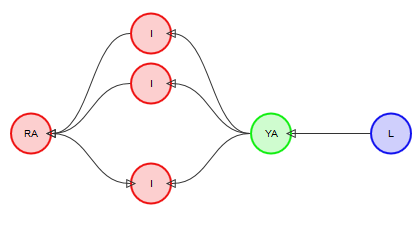
\includegraphics[scale=0.5]{./figures/graphs/aifplus.png}
\caption{Visualisation of a simple AIF+ graph}
\label{figure:graphs:aifplus}
\end{figure}

\section{Online Communication and Interaction}
\label{background:online}

\subsection{Social Media and the Social Web}
\label{background:online:social}
The social web consists of the people, tools and communities that form over the world wide web, and is a way for individuals to share content, ideas and information. The social web presents a number of challenges for extracting and analysing arguments, particularly due to the lack of clear ``indicators'' of argument or structure. This problem is compounded by the type of language used; often highly informal, incorporating slang and irregular punctuation and grammar \citep{Schneider2012}. As the social web becomes more and more ubiquitous, the potential for using it to investigate how truly massive communities interact, communicate and argue increases dramatically.

Many theoretical models of argumentation are based on the assumption of a dialectic argument, as their purpose is to aid the participants with the process of understanding the information discussed, or to reason over the model and draw conclusions regarding the outcome. However, in social media there is a clear proliferation of eristic argumentation \citep{sood2012automatic}. This makes the role of audience an important feature to consider: when an individual responds to a post on the social web their post is often seen not just by the author of the post they reply to, but by many other users as well. In fact, many posts may be directed at this wider audience to seek approval, voice dissent, or provoke other emotions \citep{berland2010students}. Consider the analogy of a political hustings: neither candidate believe they can change the mind of their opponent, but instead are debating with a view to sway their audience. Schneider et al. note though, that currently it is difficult to model the value of eristic arguments as participants are free to \textit{``sling propositions that they would not commit to under other circumstances''} as a means of catharsis, recreation or entertainment \citep{Schneider2014}.

\citet{Kaplan2010} classify six distinct categories of social media: collaborative projects, blogs, content communities, social networking sites, virtual game worlds and virtual social worlds. Collaborative projects allow many different users to create, maintain and often discuss content. This category includes sites such as the online encyclopaedia \textit{Wikipedia}\footnote{https://en.wikipedia.org/}, which allow users to write and edit articles and \textit{Urban Dictionary}\footnote{http://urbandictionary.com/‎}, a user generated dictionary of slang and internet culture. \citeauthor{Kaplan2010} compare blogs (web-logs) to personal websites, in that they allow users to post information about the subject of their choice -- these posts are often timestamped and presented reverse-chronologically. \textit{Wordpress}\footnote{http://wordpress.com/} and \textit{Blogger}\footnote{http://blogger.com} are two social media sites specialised for this purpose. ``Micro''-blogging sites that pose limits on the amount of content that can be shared in a single post, such as \textit{Twitter}\footnote{http://twitter.com/}, also fall into this category. Content communities revolve around the concept of publishing (and ultimately sharing) different forms of media. These include sites for publishing video (such as \textit{Vimeo}\footnote{http://vimeo.com/}), images (such as \textit{Flickr}\footnote{http://flickr.com/}), audio (such as \textit{SoundCloud}\footnote{http://soundcloud.com/}) and many other different types of media. Social networking sites allow users to create a profile detailing information about themselves (such as home town, or music preferences) and then connect their profiles with the profiles of others on the site. Examples include \textit{Facebook}\footnote{http://facebook.com} and \textit{Google+}\footnote{http://plus.google.com/}. Virtual game worlds (such as \textit{World of Warcraft}\footnote{http://battle.net/wow/}) encompass online games in which a user controls a digital avatar to accomplish certain tasks (such as slaying a virtual dragon, or defeating another player's avatar). Similarly, virtual social worlds (such as \textit{Second Life}\footnote{http://secondlife.com}) encompass virtual spaces in which users have an avatar, but there is no specified aim or end-goal -- the medium exists solely to facilitate social interaction. In this work, less focus is afforded to these latter two areas of the social web due to the the issue that as participants are controlling a virtual avatar, and may be playing a particular ``role'' rather than their real self, this can affect their behaviour and engagement in a discussion \cite{Hooi2013}. There is also the tendency for discussions to centre on the mechanics of the game world itself \citep{alagoz2013}.

\subsection{Anti-Social Behaviour}
\label{background:online:antisocial}
Anti-social behaviour is a growing problem on the social web, and often arises from debates or discussions that get out of hand \citep{suler1998bad, davis2002experience, sood2012automatic}. This behaviour can arise from simple misunderstandings due to the difficulty in conveying tone through text, or as a deliberate act by individuals lashing out at other participants in a discussion. Incidents include
flaming, in which a user simply hurls emotional abuse \citep[p.~13]{Konijn2008}; spamming, in which a user floods the medium with content, often unrelated to the topic in hand, in the hope of drowning out other participants or as a means of advertising a commercial product \citep{krause2008anti}; trolling, in which a user posts seemingly innocuous but deliberately fallacious argument to provoke other members of the group into becoming outraged (although there is debate as to whether this term refers to the bridge-dwelling monster of myths, or the fishing term for dangling a baited line behind a boat) \citep{Herring2002}; 
and much more serious incidents of directed threats and stalking \citep{spitzberg2002cyberstalking, willard2007, jane2014}.

As a result, there is a concerted research effort into the best way to tackle these issues before they cause serious harm to individuals, or the field as a whole. \citet{suler1998bad} discuss a wide variety of approaches (specifically in regard to the virtual social world \textit{The Palace}\footnote{http://thepalace.com}, but these could be applied to other online spaces as well). The simplest solution is to moderate users' interactions and dispense warnings, ``mutes'' (where a user may observe, but not contribute) or, in extreme cases, bans as and when the situation warrants. While effective for dealing with small or close-knit communities, this approach does not scale when considering the social web.

\TODO{Arguments against the troll} \citep{torroni2010}

A different approach is to allow the community a degree of self-moderation. Reputation systems, for example, allow users within a community to assign ``votes'' to a particular account, or post, to show its trustworthiness. This allows new users to make judgements on whether to take a comment seriously, for example, or to purchase something from a particular seller in an online auction \citep{resnick2000reputation, anderson2012discovering}. However, this can also lead to a feedback loop in which communities become self-reinforcing; if users always vote for posts of similar sentiment (or against those that disagree), then gradually these sentiments will become dominant. Over time only users who hold these views will contribute to the site (further reinforcing the disparity) and the community as a whole will stagnate or worse, become distrustful or outright hostile to new members or ``outsiders''.

In another example of direct self-moderation, the popular online game \textit{League of Legends}\footnote{http://leagueoflegends.com} implements a ``tribunal'' system in which players that are reported for poor behaviour in matches (such as verbally abusing team-mates) are judged by their peers. These peers can examine evidence such as chat logs and game scores, then decided whether to ``pardon'' or ``punish'' the offending player \citep{Hodson2013, kou2013regulating}.

A more covert attempt to manipulate users' behaviour can be found in certain implementations of human-computer interaction design. HCI can be leveraged to ``trick'' users into performing (or not performing) an action desirable to the designer. These so-called ``malicious interfaces'' \citep{Conti2010} are often used to trick users into spending time or money that they otherwise would not (for example, advertising banners that suddenly cover page content). In 2008, YouTube temporarily added an ``Audio Preview'' button to its comment system that would read aloud what the user intended to post. This was placed in the previous place of the ``post'' button (which had been moved further to the right), such that a user was likely to unintentionally preview their comment before posting it \citep{Munroe2008}.


\subsection{Semantically-Interlinked Online Communities}
%\TODO{Find some more models?}
The Semantically-Interlinked Online Communities project (SIOC) aims to enable the cross-platform, cross-service representation of data from the social web \citep{Breslin2006}. SIOC allows for semantic representations of Sites, which hold Forums, which contain Posts, authored by the owner of a UserAcount. This structure is shown in Figure \ref{figure:sioc}. SIOC is often used in conjunction with the Friend of a Friend (FOAF) ontology, to show how individuals map to their online personas.

\begin{figure}
\begin{center}
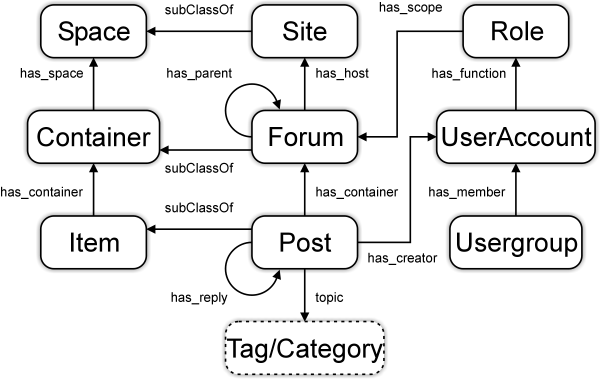
\includegraphics[scale=1.75]{./figures/ontologies/sioc.png}
\caption[An overview of the core SIOC ontology]{An overview of the core SIOC ontology\protect\footnotemark}
\label{figure:sioc}
\end{center}
\end{figure}
\footnotetext{http://sioc-project.org/ontology}

While an extension to SIOC, for the purposes of capturing and representing argumentation, does exist \citep{Lange2008}, it is based on the Issue Based Information System (IBIS) principals of modelling an argument as an issue that needs to be solved, with users suggesting ideas, then providing arguments for or arguments against these ideas. While this approach is highly useful when dealing with arguments centred around deliberation, and to a lesser extend criticism or inquiry, they are not as suitable when modelling negotiations or eristic arguments.

\section{Social Aspects of Argumentation}
\TODO{ReasonWell, etc.}

\TODO{Prescriptive vs. Descriptive etc.}

\section{Summary}
\TODO{Summarise}